\chapter{Detail Study of $\mathcal{L}_{r,c,q}$}\label{chapter:detail}

\section{Lights Out Layout}

\begin{definition}
	For every $r,c\in\N$ define the graph $\Delta_{r,c}$ with vertices
	$\{1,\ldots,r\}\times\{1,\ldots,c\}$ and edges from $(s,t)$ to $(u,v)$
	if and only if $|u-s|+|v-t| \le 1$.
		
	$\Delta_{r,c}$ is called the lights out graph with $r$ rows and $c$
	columns.
\end{definition}

\begin{definition}
	For every $r,c\in\N$ and every $q\in\N^{*}$ we define the layout
	$\mathcal{L}_{r,c,q} := \langle\Delta_{r,c},q\rangle$.
\end{definition}

\begin{theorem}
	$\mathcal{L}_{r,c,q}$ is a reflexive, symmetric layout for all
	$r,c\in\N$ and $q\in\N^{*}$.
\end{theorem}

\begin{proof}
	Let $(u,v)\in\Delta_{r,c}$, then $|u-u|+|v-v| = 0 \le 1$ hence every
	vertex is adjacent to itself so $\mathcal{L}_{r,c,q}$ is reflexive.
	
	Let $(u,v),(s,t)\in\Delta_{r,c}$. If $(s,t)$ is adjacent to $(u,v)$ then
	$|u-s| + |v-t| \le 1$ but $|u-s| + |v-t| = |s-u| + |t-v|$ so then
	$(u,v)$ is adjacent to $(s,t)$. Thus $\mathcal{L}_{r,c,q}$ is symmetric.
\end{proof}

\begin{theorem}
	$\mathcal{L}_{r,c,q}$ is chaseable for all $r,c\in\N$ and $q\in\N^{*}$.
\end{theorem}

\begin{proof}
	$(V_{i} : i \in \{1,\ldots,r\})$, where $V_{i} := \{(i,j)\in\Delta_{r,c}
	\bar j \in \{1,\ldots,c\}\}$ for all $i\in\{1,\ldots,r\}$ is a partition
	of $\Delta_{r,c}$ which satisfies properties \ref{chase:out} through
	\ref{chase:clean}.
	
	From the definition of $\Delta_{r,c}$ it is clear that $N(V_{i}) \cap
	N(V_{j}) = 0$ if $|j-i| > 1$. Furtermore every vertex $(i,y)\in V_{i}$
	has precisely one adjacent vertex in $V_{i+1}$, namely $(i+1,y)$. 
\end{proof}

\begin{example}
	We will study $\mathcal{L}_{2,3,2}$ in this example. (See also figure
	\ref{figure:graph_2,3}.) We do this by examining
	$\mathcal{L}_{2,3,2}\down$.
	\begin{figure}
		\begin{center}
			\includegraphics{image/graph.3}
		\end{center}
		\caption{$\Delta_{2,3}$ depicted as a graph.}\label{figure:graph_2,3}
	\end{figure}
	
	When button $(1,1)$ is pressed the following buttons light up: $(1,1)$,
	$(1,2)$ and $(2,1)$. In order to chase this pattern down one has to
	press buttons $(2,1)$ and $(2,2)$. All buttons in the first row are now
	unlit. 
	
	Button $(2,1)$ has changed it state an odd number of times. (It	changes
	state every button press.) So button $(2,1)$ is lit. Button $(2,2)$
	changed state an even number of times so it is unlit. The last button,
	$(2,3)$, is lit. This tells use what the chased down light pattern is.
	(It tells us $\overline{(1,1)}\down$.) By symmetry we also know
	$\overline{(1,3)}\down$. It is the mirror image of
	$\overline{(1,1)}\down$. In particular is it identical to
	$\overline{(1,1)}\down$. When chasing down $\overline{(1,2)}$ we come to
	the conclusion that $\overline{(1,2)}\down=O$.
	
	We now know $\mathcal{L}_{2,3,2}\down$.
	$\Gamma_{\mathcal{L}_{2,3,2}\down}$ has three vertices and the following
	adjacency matrix (See also figure \ref{figure:graph_2,3down}.)
	\begin{figure}
		\begin{center}
			\includegraphics{image/graph.3}
		\end{center}
		\caption{$\Delta_{2,3}$ depicted as a graph.}\label{figure:graph_2,3down}
	\end{figure}
	\[
		\left(
		\begin{array}{ccc}
			1 & 0 & 1 \\
			0 & 0 & 0 \\
			1 & 0 & 1 \\
		\end{array}
		\right)
	\]
	
	$\Im(I_{\mathcal{L}_{2,3,2}\down})$ is spanned by $(1,0,1)^{t}$.
	$\Ker(I_{\mathcal{L}_{2,3,2}\down})$ is spanned by $(0,1,0)^{t}$ and
	$(1,0,1)^{t}$.
\end{example}

\section{Windowing}

In order to adress questions of solvability of states in $\mathcal{L}_{r,c,q}$,
the general theory developed in chapter \ref{chapter:mathematics} suggests tot
look at $\mathcal{L}_{r,c,q}\down$. Because (almost) every row acts the same on
the preceding row, we can develop a windowing algorithm.
\begin{figure}
	\begin{center}
		\hspace*{\fill}
		\subfigure[First window]{\includegraphics[width=35mm]{image/windowing1.ps}}
		\hfill
		\subfigure[Second window]{\includegraphics[width=35mm]{image/windowing2.ps}}
		\hspace*{\fill}
	\end{center}
	\caption{Windowing.}\label{figure:windowing}
\end{figure}

When chasing a lights out layout $\mathcal{L}_{r,c,q}$ it is clear that lit
buttons only occure in a window of depth two. Suppose that only buttons in the
first row are pressed. The effect of these presses does not reach beyond row
two. If the buttons in the second row of the press pattern which chases this
light pattern down are pressed, only buttons in row two and three can be lit.
(All buttons are unlit by design and buttons in row two do not effect buttons
beyond row three.)

We can confine our attention to a window of depth two. (See also figure
\ref{figure:windowing}.) The next window is completely determined by
the current window. 

By pretending there are imaginary rows before and after our real rows, the
discription of windowing is particularly nice.

\begin{definition}
	Define $2c \times 2c$ matrix $W_{c,q}$ with entries in $\Z/q\Z$ to be
	the matrix
	\[
		\left(
		\begin{array}{cc}
			E_{c} & I_{c} \\
			I_{c} & O_{c} \\			
		\end{array}
		\right)
	\]
	where $O_{c}$ and $I_{c}$ are the $c \times c$ zero and identy matrix
	respectively and $E_{c}$ is the matrix with a block of three
	consecutive ones in row $1 < i < c$ starting in column $i-1$ and a block
	of two consecutive ones in row $1$ starting in column 1 and in row $c$
	starting in column $c-1$. (See also table \ref{table:E} for $E_{5}$.)
	\begin{table}
		\[
		\left(
		\begin{array}{ccccc}
			1 & 1 & 0 & 0 & 0 \\
			1 & 1 & 1 & 0 & 0 \\
			0 & 1 & 1 & 1 & 0 \\
			0 & 0 & 1 & 1 & 1 \\
			0 & 0 & 0 & 1 & 1 \\
		\end{array}
		\right)
		\]
		\caption{$E_{5}$}\label{table:E}
	\end{table}
	
	The above definition for $E_{c}$ is not clear when $c=1$ or $c=2$.
	$E_{1} := \left(1\right)$ and
	\[
		E_{2} := \left(
		\begin{array}{cc}
			1 & 1 \\
			1 & 1 \\
		\end{array}
		\right)		
	\]
\end{definition}

\begin{lemma}
	$\det(W_{c}) = (-1)^{c}$.
\end{lemma}

\begin{proof}
	We will proof that $\det(W_{c,q}) = (-1)^c$ using induction on $c$.
	Notice that
	\[
		\det W_{1} = \det \left(
		\begin{array}{cc}
			1 & 1 \\
			1 & 0 \\
		\end{array}
		\right) = -1
	\]
	
	Now developing the determinant of $W_{c+1}$ along row $c+1$ and
	column $c+1$ shows that	$\det(W_{c+1}) = (-1)^{(c+1)}(-1)^{c}
	\det(W_{c}) = -\det(W_{c})$.
	
	By induction it is shown that $\det(W_{c}) = (-1)^{c}$.
\end{proof}

\begin{lemma}\label{lemma:Winverse}
	The inverse for $W_{c}$ is
	\[
 		\left(
		\begin{array}{cc}
			0 & I      \\
			I & -E_{c} \\
		\end{array}
		\right)
	\]
\end{lemma}

\begin{proof}
	\[
 		\left(
		\begin{array}{cc}
			E & I \\
			I & 0 \\
		\end{array}
		\right)		
 		\left(
		\begin{array}{cc}
			0 & I  \\
			I & -E \\
		\end{array}
		\right)
		=
 		\left(
		\begin{array}{cc}
			E \cdot 0 + I \cdot I & E \cdot I + I \cdot -E \\
			I \cdot 0 + 0 \cdot I & I \cdot I + 0 \cdot -E \\
		\end{array}
		\right)
		=
 		\left(
		\begin{array}{cc}
			I & 0 \\
			0 & I \\
		\end{array}
		\right)		
	\]
\end{proof}

\begin{corollary}\label{corollary:Wperiodic}
	The sequence $(W_{c}^{n})_{n\in\N}$ is periodic.
\end{corollary}

\begin{proof}
	Let $W := W_{c}$.
	
	Notice that there are only finitelly many $2c \times 2c$ matrices with
	entries in $\Z/q\Z$. So there will $s$ and $t$ in $\N$ such that $s<t$
	such that $W^{s} = W^{t}$. Choose $s$ and $t$ such that $s$ and $t-s$
	are as small as possible. Because $W$ is invertible $s=0$. (Otherwise
	$W^{s-1} = W^{-1} W^{s} = W^{-1} W^{t} = W^{t-1}$ and then $s-1$, $t-1$
	would be a smaller pair.)
	
	The sequence $(W_{c}^{n})_{n\in\N}$ is seen to be periodic with period
	$t$.
\end{proof}

Now that we have defined $W_{c}$ we can study the dimension of the kernel of
$I_{\mathcal{L}_{c,r,q}}$.

\section{Dimension of Kernel of $I_{\mathcal{L}_{c,r,q}}$}

\begin{theorem}
	The sequence $(\dim(\Ker(I_{\mathcal{L}_{r,c,q}})))_{r\in\N}$ is
	periodic for all $c,q\in \N$. 	
\end{theorem}

\begin{proof}
	The sequence is determined by the upper left $c \times c$ submatrix of
	$W_{c}^r$. According to corallary \ref{corollary:Wperiodic} $W_{c,q}$ is
	periodic.
\end{proof}

\begin{lemma}
	Let $v\in \Ker(I_{\mathcal{L}_{c,r,q}})$ be non-trivial, then at least
	one of the first $c$ button is pressed.
\end{lemma}

\begin{proof}
	Let $v\in\Ker(I_{\mathcal{L}_{c,r,q}})$ be a non-trivial element. If
	neither of the buttons in the first row gets pressed, none of the
	buttons in this rows is lit. By	considering our chasing algorithme it is
	clear that other buttons also do not get pressed.
	
	So no button gets pressed contrary to our assumption.
\end{proof}

\begin{proposition}\label{proposition:WpowerI}
	For all $c\in\N$, $q\in\N^{*}$ there exists an $r\in\N$ such that
	\[
		\dim(\Ker(I_{\mathcal{L}_{r,c,q}})) = c
	\]
\end{proposition}

\begin{proof}
	There exist a $r\in\N^{*}$ such that $W_{c}^{r+1} = I$. So $W_{c}^{r} =
	W_{c}^{-1}W_{c}^{r+1} = W_{c}^{-1}$. By lemma \ref{lemma:Winverse} we
	know that the upper left square of $W_{c}^{-1}$ is the zero matrix.
	
	Because every row of this (sub)matrix determines the $\overline{b}\down$
	for every button in the first row of buttons. We have $c$ independent
	elements in $\Ker(I_{\mathcal{L}_{r,c,q}})$.
\end{proof}

\begin{corollary}
	If $\dim(\Ker(I_{\mathcal{L}_{r,c,q}})) = c$, then
	$\dim(\Ker(I_{\mathcal{L}_{r+1,c,q}})) = 0$. 
\end{corollary}

\begin{proof}
	This is clear from the preceding proof.
\end{proof}

\begin{proposition}
	If $\dim(\Ker(I_{\mathcal{L}_{r,c,q}})) = c$, then
	$\dim(\Ker(I_{\mathcal{L}_{r-1,c,q}})) = 0$.
\end{proposition}

\begin{proof}
	The assertion follows from theorem \ref{proposition:WpowerI} and lemma
	\ref{lemma:Winverse}.
\end{proof}

\begin{proposition}
	If $\dim(\Ker(I_{\mathcal{L}_{r,c,q}})) = c$ and $t,t'\in\N^{*}$ such
	that $t + 1 + t' = r$ then
	\[
		\dim(\Ker(I_{\mathcal{L}_{t,c,q}})) = \dim(\Ker(I_{\mathcal{L}_{t',c,q}}))
	\]
\end{proposition}

\begin{proof}
	Because every button press in the first row can be extended to a element
	of $\Ker(I_{\mathcal{L}_{r,c,q}})$.
\end{proof}
